%---------------------- % % % Personnalisation des couleurs % % % ---------- GRIS -------
\definecolor{couleurFonce}{RGB}{110,110,110} % Couleur du Code APOGEE
\definecolor{couleurClaire}{RGB}{205,205,205} % Couleur du fond de la bande
\definecolor{couleurTexte}{RGB}{255,255,255} % Couleur du texte de la bande
%------------------------------------------------------------------------------------------


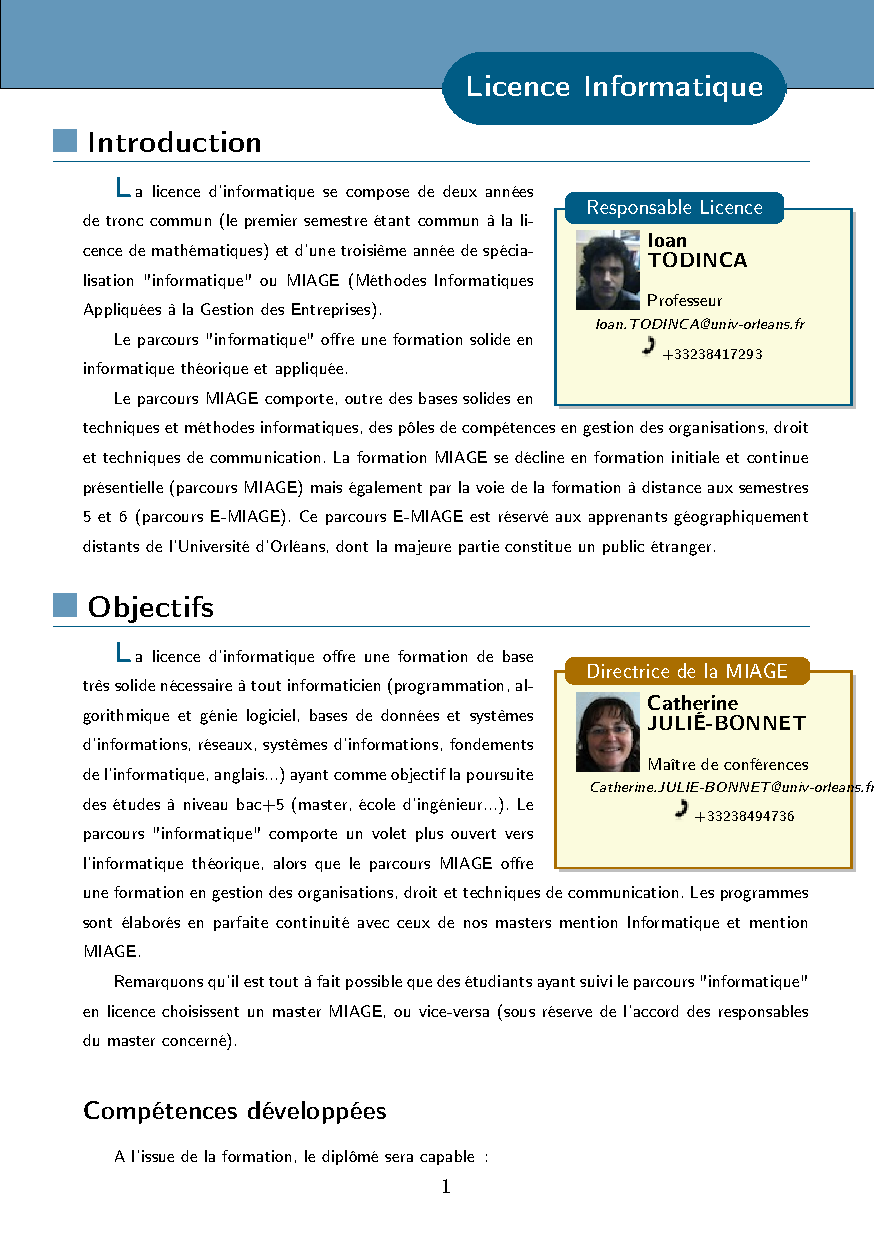
\includepdf[fitpaper,pages=-]{Preambule_Info_MasterVIP_S3S4.pdf}

%==========================================================================================
% SEMESTRE 3
%==========================================================================================
\module[codeApogee={UE 31 }, 
titre={Informatique ambiante}, 
CODEUE={1}, 
COURS={61}, 
TD={}, 
TP={64}, 
CTD={}, 
TOTAL={125}, 
SEMESTRE={Semestre 3}, 
COEFF={10}, 
ECTS={10}, 
MethodeEval={Contrôle continue et terminal}, 
ModalitesCCSemestreUn={CC et CT}, 
ModalitesCCSemestreDeux={CT}, 
%CalculNFSessionUne={$\frac{(CC+2*CT)}{3}$}, 
%CalculNFSessionDeux={CT}, 
NoteEliminatoire={7}, 
nomPremierResp={Rémy LECOGNE}, 
emailPremierResp={Remy.LECOGNE@univ-orleans.fr}, 
nomSecondResp={}, 
emailSecondResp={}, 
langue={Français}, 
nbPrerequis={0}, 
descriptionCourte={true}, 
descriptionLongue={true}, 
objectifs={true}, 
ressources={true}, 
bibliographie={false}] 
{
Unité orbligatoire.\\
Cette unité se passe sur le site de l\'école Polytech\'Orléans dans la spécialité "
} 
{
\begin{enumerate}
\item Réseaux de communication
 \begin{itemize}
 \item Connaitre les différentes technologies de communication sans fil.
 \item Sélectionner la technologie la plus adaptée à une situation donnée.
 \item Mettre en place un système de communication sans fils (Bluetooth, Wifi, RFID, ....).
 \item Identifier les différents systèmes d\'exploitation et leurs limites (cas des systèmes mobiles).
 \end{itemize} 
\item Informatique Graphique
 \begin{itemize}
 \item Comprendre les architectures (matérielles et logicielles) permettant une programmation parallèle.
 \item Réaliser des programmes déployés sur GPU.
 \item Mettre en place des interfaces ergonomiques.
 \item Utiliser les bibliothèques usuelles de génération et de visualisation de graphismes 2D et 3D.
 \end{itemize} 
\item Design logiciel
 \begin{itemize}
 \item Comprendre et appliquer les méthodes de conception et de qualité logicielle.
 \item Mettre en \oe uvre des procédures de test logiciel.
 \item Connaitre les failles de sécurité liées au développement logiciel ou aux réseaux de communication.
 \end{itemize}
\end{enumerate}
} 
{} 
{\begin{itemize}
\ObjItem Comprendre et mettre en place des transferts de données via des réseaux de communication sans fils.
\ObjItem Réaliser des programmes bien construits, fiables et sécurisés.
\ObjItem Maitriser les architectures et programmations parallèles.
\ObjItem Mettre en en place des programmes ergonomiques et visuels (utilisation de graphismes 2D ou 3D).
\end{itemize} 
} 
{Ressources} 
{Biblio} 
 
\vfill

%==========================================================================================
\module[codeApogee={UE 32}, 
titre={Imagerie opérationnelle}, 
CODEUE={1}, 
COURS={74}, 
TD={51}, 
TP={}, 
CTD={}, 
TOTAL={125}, 
SEMESTRE={Semestre 3}, 
COEFF={10}, 
ECTS={10}, 
MethodeEval={Contrôle continue et terminal}, 
ModalitesCCSemestreUn={CC et CT}, 
ModalitesCCSemestreDeux={CT}, 
%CalculNFSessionUne={$\frac{(CC+2*CT)}{3}$}, 
%CalculNFSessionDeux={CT}, 
NoteEliminatoire={7}, 
nomPremierResp={Rachid JENNANE}, 
emailPremierResp={Rachid.JENNANE@univ-orleans.fr}, 
nomSecondResp={}, 
emailSecondResp={}, 
langue={Français}, 
nbPrerequis={0}, 
descriptionCourte={true}, 
descriptionLongue={true}, 
objectifs={true}, 
ressources={true}, 
bibliographie={false}] 
{
Unité orbligatoire.\\
Cette unité se passe sur le site de l\'école Polytech\'Orléans dans la spécialité "Écotechnologies Électroniques et Optiques". 
} 
{
\begin{enumerate}
\item Analyse d\'images
 \begin{itemize}
 \item Choisir les outils logiciels adaptés à une problématique
 \item Savoir segmenter une image
 \item Résoudre un problème mal posé par des méthodes inverses
 \item Détecter des contours par modèles déformables
 \item Reconnaitre des formes dans une image
 \item Classifier des objets dans des bases d\'images
 \item Tatouer une image pour cacher des informations
 \item Synthétiser des images texturées
 \end{itemize}
\item Traitements vidéo
 \begin{itemize}
 \item Indexer une vidéo par le contenu
 \item Analyser une séquence vidéo
 \item Suivre une cible dans une séquence vidéo
 \item Modéliser la prise de vue et le déplacement d\'une caméra 
 \item Faire un panorama avec une mosaïque d\'images
 \item Exploiter la réalité augmentée 
 \item Reconstruire des objets 3D par tomographie 
 \end{itemize}
\item Tests, contrôle et validation
 \begin{itemize}
 \item Analyse multivariable (ACP) et réduction de dimensionnalité
 \item Savoir choisir des vecteurs tests, une base de données, une vérité terrain
 \item Choisir des critères de validation
 \item Réaliser un plan de contrôles
 \end{itemize}
\item Fusion de données
 \begin{itemize}
 \item Fusionner des données par approches probabiliste, floue et fonctions de croyance
 \item Traiter des données sur GPU pour télévision 3D
 \item Embarquer un traitement d\'image 
 \item Traiter des images couleurs
 \item Fouille de données pour l\'extraction de connaissances
 \end{itemize}
\end{enumerate}
} 
{} 
{\begin{itemize}
\ObjItem Maîtriser les aspects théoriques des méthodes de traitement des images.
\ObjItem Être capable de d\'établir des plans de tests pertinents pour valider les techniques de vision et d\'imagerie mises en \oe uvre.
\ObjItem Être capable de fusionner les informations en provenance de différents capteurs et savoir prendre des décisions.
\ObjItem Objectif
\end{itemize} 
} 
{Ressources} 
{Biblio} 
 
\vfill

%==========================================================================================
\module[codeApogee={UE 33 }, 
titre={Management opérationnel}, 
CODEUE={1}, 
COURS={16}, 
TD={24}, 
TP={16}, 
CTD={}, 
TOTAL={56}, 
SEMESTRE={Semestre 3}, 
COEFF={4}, 
ECTS={4}, 
MethodeEval={Contrôle continue et terminal}, 
ModalitesCCSemestreUn={CC et CT}, 
ModalitesCCSemestreDeux={CT}, 
%CalculNFSessionUne={$\frac{(CC+2*CT)}{3}$}, 
%CalculNFSessionDeux={CT}, 
NoteEliminatoire={7}, 
nomPremierResp={Jean-Jacques YVERNAULT}, 
emailPremierResp={Jean-Jacques.YVERNAULT@univ-orleans.fr}, 
nomSecondResp={}, 
emailSecondResp={}, 
langue={Français}, 
nbPrerequis={0}, 
descriptionCourte={true}, 
descriptionLongue={true}, 
objectifs={true}, 
ressources={true}, 
bibliographie={false}] 
{
Unité orbligatoire.\\
Cette unité se passe sur le site de l\'école Polytech\'Orléans. 
} 
{
\begin{description}
\item[Rôle et missions]
Styles de management et évolution des missions de l\'ingénieur. La notion de responsabilité d\'un poste. 
La relation client-fournisseur interne et l\'arbitrage. La relation client-fournisseur externe : négocier des achats des ventes.
Les liens entre le stage d\'ingénieur et le management.
\item[Travailler en équipe]
Typologie des comportements au sein d\'une équipe. Réunions d\'information et de résolution de problèmes. 
Entretiens de management et d\'évaluation. Donner des directives. Motiver ses collègues. Gérer les cas difficiles et les conflits. 
S\'organiser, faire le suivi. Gérer le stress.
\item[Management de la qualité et du développement durable]
Méthodes et outils du management de qualité et de la résolution de problème. Développement durable : 
démarche intégrée, indicateur et prévention des risques.
\end{description}
} 
{} 
{\begin{itemize}
\ObjItem Optimiser son comportement, son relationnel et son organisation pour tenir et développer son rôle d\'ingénieur au sein d\'une entreprise.
\ObjItem Acquérir les méthodes de l\'animation d\'équipe et de la négociation.
\ObjItem Comprendre les ressorts de la motivation.
\ObjItem Participer aux réunions et entretiens avec efficacité.
\ObjItem Utiliser les outils de management de la qualité et du développement durable.
\ObjItem Valoriser son stage.
\end{itemize} 
} 
{Ressources} 
{Biblio} 
 
\vfill

%==========================================================================================
\module[codeApogee={UE 34}, 
titre={Simulation et stratégie d\'entreprise}, 
CODEUE={1}, 
COURS={}, 
TD={24}, 
TP={}, 
CTD={}, 
TOTAL={24}, 
SEMESTRE={Semestre 3}, 
COEFF={3}, 
ECTS={3}, 
MethodeEval={Contrôle continue et terminal}, 
ModalitesCCSemestreUn={CC et CT}, 
ModalitesCCSemestreDeux={CT}, 
%CalculNFSessionUne={$\frac{(CC+2*CT)}{3}$}, 
%CalculNFSessionDeux={CT}, 
NoteEliminatoire={7}, 
nomPremierResp={Chaker HAOUET}, 
emailPremierResp={Chaker.HAOUET@univ-orleans.fr}, 
nomSecondResp={}, 
emailSecondResp={}, 
langue={Français}, 
nbPrerequis={0}, 
descriptionCourte={true}, 
descriptionLongue={true}, 
objectifs={true}, 
ressources={true}, 
bibliographie={false}] 
{
Unité obligatoire. 
} 
{
Les étudiants sont mis en situation de gérer une entreprise à travaers des décisions d\'ordre commercial, financier et de production. Ces entreprises sont en concurrence sur le marché, et sont en mesure d\'évaluer régulièrement leurs résultats à l\'aide des documents financiers et d\'études de positionnement. Ainsi cette situation de gestion d\'entreprise est l\'occasion d\'appliquer les principaux concepts en statégies et marketing, et d\'élaborer des tableaux de bord afin de guider les étudiants dans leurs décisions et d\'en mesurer les impacts financier. 
} 
{} 
{\begin{itemize}
\ObjItem Connaissance du monde de l\'entreprise.
\end{itemize} 
} 
{Ressources} 
{Biblio} 
 
\vfill

%==========================================================================================
\module[codeApogee={UE 35}, 
titre={Initiation à la recherche}, 
CODEUE={1}, 
COURS={57}, 
TD={}, 
TP={}, 
CTD={}, 
TOTAL={57}, 
SEMESTRE={Semestre 3}, 
COEFF={7}, 
ECTS={7}, 
MethodeEval={Contrôle continue et terminal}, 
ModalitesCCSemestreUn={CC et CT}, 
ModalitesCCSemestreDeux={CT}, 
%CalculNFSessionUne={$\frac{(CC+2*CT)}{3}$}, 
%CalculNFSessionDeux={CT}, 
NoteEliminatoire={7}, 
nomPremierResp={Sophie ROBERT}, 
emailPremierResp={Sophie.ROBERT@univ-orleans.fr}, 
nomSecondResp={Rachid JENNANE}, 
emailSecondResp={Rachid.JENNANE@univ-orleans.fr}, 
langue={Français}, 
nbPrerequis={1}, 
descriptionCourte={true}, 
descriptionLongue={true}, 
objectifs={true}, 
ressources={true}, 
bibliographie={false}] 
{
Unité conseillée pour ceux qui se destinent à la recherche.
} 
{
Initiation au stage recherche :
\begin{itemize}
\item introduction d\'outils pour aborder un stage de recherche en laboratoire
\item présentation du cycle de tutoriaux, des thématiques, des possibilités de poursuites en thèse et plus largement du milieu de la recherche académique ou industrielle
\item présentation des projets académiques proposés au semestre 4
\end{itemize} 
Cycle de tutoriaux :
\begin{itemize}
\item 2 tutoriaux longs (d\'une durée totale de 9h; soit 2 fois 3 séances de 1h30) seront axés sur une thématique préalablement
choisie et pour laquelle un renforcement est sollicité par le laboratoire.
\item 20 tutoriaux courts (de 1h30 chacun) articulés autour de thématiques telles que la résolution par contraintes,
l\'apprentissage, extraction de connaissances, le parallélisme, la réalité virtuelle, la sécurité et sûreté des logiciels,
les modèles de calculs, l\'algorithmique et la théorie des graphes, ...
\end{itemize} 
Ces tutoriaux se voudront à la fois introductifs et concrets, mais ils apporteront également des connaissances pointues sur des domaines maîtrisés par les intervenants. 
}
{Avoir une connaissance générale de l\'informatique.}
{\begin{itemize}
\ObjItem L\'objectif est d\'initier l\'étudiant à une démarche scientifique et de le familiariser à un travail de recherche bibliographique. 
\ObjItem Les tutoriaux ont pour objectif d\'appréhender quelques thématiques de recherche et d\'introduire des techniques récentes ou fondamentales.
\end{itemize} 
} 
{Ressources} 
{Biblio} 
 
\vfill

%==========================================================================================
\module[codeApogee={UE 36}, 
titre={Projet}, 
CODEUE={1}, 
COURS={}, 
TD={}, 
TP={}, 
CTD={}, 
TOTAL={}, 
SEMESTRE={Semestre 3}, 
COEFF={3}, 
ECTS={3}, 
MethodeEval={Contrôle continue et terminal}, 
ModalitesCCSemestreUn={Rapport et soutenance de projet}, 
ModalitesCCSemestreDeux={CT}, 
%CalculNFSessionUne={$\frac{(CC+2*CT)}{3}$}, 
%CalculNFSessionDeux={CT}, 
NoteEliminatoire={7}, 
nomPremierResp={Sophie ROBERT}, 
emailPremierResp={Sophie.ROBERT@univ-orleans.fr}, 
nomSecondResp={Rachid JENNANE}, 
emailSecondResp={Rachid.JENNANE@univ-orleans.fr}, 
langue={Français}, 
nbPrerequis={1}, 
descriptionCourte={true}, 
descriptionLongue={true}, 
objectifs={true}, 
ressources={true}, 
bibliographie={false}] 
{
} 
{
Réalisation d\'une application en rapport avec les UE du semestre. 
} 
{Maîtrise des techniques de développement de logiciels.} 
{\begin{itemize}
\ObjItem Mise en pratique des principes et techniques étudiés dans les unités d\'enseignement.
\end{itemize} 
} 
{Ressources} 
{Biblio} 
 
\vfill

%==========================================================================================
% SEMESTRE 4
%==========================================================================================
\module[codeApogee={UE 41}, 
titre={Programmation multi-c\oe urs}, 
CODEUE={1}, 
COURS={20}, 
TD={15}, 
TP={}, 
CTD={}, 
TOTAL={35}, 
SEMESTRE={Semestre 4}, 
COEFF={3}, 
ECTS={3}, 
MethodeEval={Contrôle continue et terminal}, 
ModalitesCCSemestreUn={CC et CT}, 
ModalitesCCSemestreDeux={CT}, 
%CalculNFSessionUne={$\frac{(CC+2*CT)}{3}$}, 
%CalculNFSessionDeux={CT}, 
NoteEliminatoire={7}, 
nomPremierResp={Sylvain JUBERTIE}, 
emailPremierResp={Sylvain.JUBERTIE@univ-orleans.fr}, 
nomSecondResp={}, 
emailSecondResp={}, 
langue={Français}, 
nbPrerequis={1}, 
descriptionCourte={true}, 
descriptionLongue={true}, 
objectifs={true}, 
ressources={true}, 
bibliographie={false}] 
{
Unité obligatoire. 
} 
{
Ce cours porte sur l\'exploitation des différents niveaux de parallélisme présents dans la quasi-totalité des architectures actuelles. Ces niveaux (multi-coeurs, unités vectorielles et cartes graphiques) seront d\'abord présentés, en particulier, les problématiques de programmation liées aux spécificités de ces architectures seront étudiés (hyperthreading, pipeline, cache, modèle mémoire, alignement).
Après une introduction aux structures de données adaptées au parallélisme en mémoire partagée, la programmation de ces architectures sera étudiée au travers d\'exemples touchant au calcul scientifique et au traitement d\'images. La programmation des processeurs multi-coeurs reposera sur l\'utilisation des Pthreads, d\'OpenMP, d\'Intel TBB et sur une présentation du concept de transaction. La programmation de cartes graphiques reposera sur l\'utilisation de CUDA et les jeux d\'instructions SSE et Altivec seront utilisés pour la programmation des unités vectorielles intégrées dans les processeurs. Une vision plus
haut-niveau sera donnée au travers de la librairie OpenCL. Finalement, l\'accent sera mis sur la combinaison de ces différents niveaux de parallélisme, la mesure des performances et l\'adéquation
entre problèmes et choix d\'architectures/algorithmes adaptés. 
} 
{Programmation impérative
Architecture des ordinateur} 
{\begin{itemize}
\ObjItem Capacité à exploiter correctement et efficacement les différents niveau de parallèlisme présents dans les architectures actuelles.
\ObjItem Capacité à choisir une architecture en fonction d\'un problème donné.
\ObjItem Capacité à utiliser ces compétences dans les domaines du calcul scientifique et du traitement d\'images.
\end{itemize} 
} 
{Ressources} 
{Biblio} 
 
\vfill

%==========================================================================================
\module[codeApogee={UE 42}, 
titre={Visualisation avancée}, 
CODEUE={1}, 
COURS={20}, 
TD={15}, 
TP={}, 
CTD={}, 
TOTAL={35}, 
SEMESTRE={Semestre 4}, 
COEFF={3}, 
ECTS={3}, 
MethodeEval={Contrôle continue et terminal}, 
ModalitesCCSemestreUn={CC et CT}, 
ModalitesCCSemestreDeux={CT}, 
%CalculNFSessionUne={$\frac{(CC+2*CT)}{3}$}, 
%CalculNFSessionDeux={CT}, 
NoteEliminatoire={7}, 
nomPremierResp={Sébastien LIMET}, 
emailPremierResp={Sebastien.LIMET@univ-orleans.fr}, 
nomSecondResp={}, 
emailSecondResp={}, 
langue={Français}, 
nbPrerequis={0}, 
descriptionCourte={true}, 
descriptionLongue={true}, 
objectifs={true}, 
ressources={true}, 
bibliographie={false}] 
{
Unité obligatoire. 
} 
{
La complexité sémantique et la massivité des données issues de mesures scientifiques, de simulations numériques ou d\'immenses bases de données disponibles sur le réseau, rendent indispensable le recours à la médiation visuelle pour en permettre une appréhension la plus riche possible.  La mise en oeuvre de  techniques de visualisation élaborées conduit à utiliser des architectures parallèles et distribués pour faire face à la complexité des traitements numériques en amont ou propre au rendu visuel. Cette puissance de traitement peut être mise en oeuvre pour simplifier le rendu afin de l\'adapter à un rendu nomade, mais elle  peut aussi adapter les données en post-traitement pour que celles-ci soient analysées via un vaste environnement de Réalité Virtuelle multi-écrans plus ou moins distant sur le réseau.
Nous présentons dans ce cours  les fondements du pipeline graphique parallèle, les différentes techniques de rendu scientifique, les moyens d\'adapter le rendu nomade aux gros volumes de données complexes et enfin nous abordons la visualisation scientifique utilisant les techniques avancée de Réalité Virtuelle au service de la performance. 
} 
{Module Calcul intensif, Module programmation graphique. Notions en Réseaux.Architecture des systèmes} 
{\begin{itemize}
\ObjItem Comprendre différentes techniques de visualisation d\'information scientifique. Comprendre le fonctionnement d\'une application graphique nomade.
\ObjItem Aborder sur des exemples les principes des applications  de visualisation scientifique portants sur des données massives de type geo-scientifique ou biologie moléculaire.
\end{itemize} 
} 
{Ressources} 
{Biblio} 
 
\vfill

%==========================================================================================
\module[codeApogee={UE 43}, 
titre={Fouille d\'images}, 
CODEUE={1}, 
COURS={20}, 
TD={15}, 
TP={}, 
CTD={}, 
TOTAL={35}, 
SEMESTRE={Semestre 4}, 
COEFF={3}, 
ECTS={3}, 
MethodeEval={Contrôle continue et terminal}, 
ModalitesCCSemestreUn={CC et CT}, 
ModalitesCCSemestreDeux={CT}, 
%CalculNFSessionUne={$\frac{(CC+2*CT)}{3}$}, 
%CalculNFSessionDeux={CT}, 
NoteEliminatoire={7}, 
nomPremierResp={Christel VRAIN}, 
emailPremierResp={Christel.VRAIN@univ-orleans.fr}, 
nomSecondResp={}, 
emailSecondResp={}, 
langue={Français}, 
nbPrerequis={1}, 
descriptionCourte={true}, 
descriptionLongue={true}, 
objectifs={true}, 
ressources={true}, 
bibliographie={false}] 
{
Unité obligatoire.
} 
{
Ce module explore les différentes techniques et compétences nécessaires à la fouille d\'images, depuis la description synthétique des images jusqu\'aux techniques d\'apprentissage automatique.
La description synthétique des images consiste à extraire un nombre restreint de descripteurs numériques, représentatifs du contenu de l\'image, la décrivant sur un plan local ou global (orientations ou couleurs dominantes, texture...). Nous étudierons ou rappellerons différentes méthodes d\'extraction de descripteurs, tels que les histogrammes, les matrices de cooccurence ou encore les ondelettes. Nous verrons également comment extraire les points d\'intérêt au sein des images.
Par ailleurs, nous présenterons différentes facettes de l\'apprentissage automatique, d\'abord de manière générale, puis dans le cadre de leur application aux images.
Nous aborderons la notion de distance ou similarité, nous montrerons comment elle peut s\'appliquer pour des recherches locales (images similaires, classification par plus proche voisin...) ou globale (structuration de l\'espace des images, clustering...).
Nous étudierons l\'impact de connaissances a priori sur l\'efficacité des méthodes (approches non supervisées, supervisées, semi-supervisées). 
} 
{} 
{\begin{itemize}
\ObjItem Apporter à l\'étudiant une double compétence dans les techniques d\'apprentissage en général et dans leur application aux images en particulier.
\end{itemize} 
} 
{Ressources} 
{Biblio} 
 
\vfill

%==========================================================================================
\module[codeApogee={UE 44}, 
titre={Préparation au stage recherche}, 
CODEUE={1}, 
COURS={}, 
TD={}, 
TP={}, 
CTD={}, 
TOTAL={}, 
SEMESTRE={Semestre 4}, 
COEFF={6}, 
ECTS={6}, 
MethodeEval={Contrôle continue et terminal}, 
ModalitesCCSemestreUn={Rapport et soutenance de projet}, 
ModalitesCCSemestreDeux={CT}, 
%CalculNFSessionUne={$\frac{(CC+2*CT)}{3}$}, 
%CalculNFSessionDeux={CT}, 
NoteEliminatoire={7}, 
nomPremierResp={Prénom NAAAAOM}, 
emailPremierResp={Prenom.NOM@univ-orleans.fr}, 
nomSecondResp={}, 
emailSecondResp={}, 
langue={Français}, 
nbPrerequis={0}, 
descriptionCourte={true}, 
descriptionLongue={true}, 
objectifs={true}, 
ressources={true}, 
bibliographie={false}] 
{
Unité conseillée pour ceux qui se destinent à la recherche.
} 
{
\begin{itemize}
\item Réalisation d\'un état de l\'art ou/et d\'une expérimentation dans un domaine précis de l\'informatique.
\item Initiation à la recherche.
\end{itemize} 
Les étudiants assistent à 4h de cours pour avoir les prérequis pour ce module.
}
{}
{\begin{itemize}
\ObjItem Savoir réaliser un état de l\'art dans un domaine spécialisé de la recherche en informatique et être à même d\'amorcer une démarche scientifique.
\end{itemize} 
} 
{Ressources} 
{Biblio} 
 
\vfill

%==========================================================================================
\module[codeApogee={UE 45}, 
titre={Projet}, 
CODEUE={1}, 
COURS={}, 
TD={}, 
TP={}, 
CTD={}, 
TOTAL={}, 
SEMESTRE={Semestre 4}, 
COEFF={6}, 
ECTS={6}, 
MethodeEval={Contrôle continue et terminal}, 
ModalitesCCSemestreUn={Rapport et soutenance de projet}, 
ModalitesCCSemestreDeux={CT}, 
%CalculNFSessionUne={$\frac{(CC+2*CT)}{3}$}, 
%CalculNFSessionDeux={CT}, 
NoteEliminatoire={7}, 
nomPremierResp={Sophie ROBERT}, 
emailPremierResp={Sophie.ROBERT@univ-orleans.fr}, 
nomSecondResp={Rachid JENNANE}, 
emailSecondResp={Rachid.JENNANE@univ-orleans.fr}, 
langue={Français}, 
nbPrerequis={1}, 
descriptionCourte={true}, 
descriptionLongue={true}, 
objectifs={true}, 
ressources={true}, 
bibliographie={false}] 
{
} 
{
Réalisation d\'une application en rapport avec les UE du semestre. 
} 
{Maîtrise des techniques de développement de logiciels.} 
{\begin{itemize}
\ObjItem Mise en pratique des principes et techniques étudiés dans les unités d\'enseignement.
\end{itemize} 
} 
{Ressources} 
{Biblio} 
 
\vfill

%==========================================================================================
\module[codeApogee={UE 46}, 
titre={Anglais}, 
CODEUE={1}, 
COURS={}, 
TD={24}, 
TP={}, 
CTD={}, 
TOTAL={24}, 
SEMESTRE={Semestre 4}, 
COEFF={3}, 
ECTS={3}, 
MethodeEval={Contrôle continue et terminal}, 
ModalitesCCSemestreUn={CC et CT}, 
ModalitesCCSemestreDeux={CT}, 
%CalculNFSessionUne={$\frac{(CC+2*CT)}{3}$}, 
%CalculNFSessionDeux={CT}, 
NoteEliminatoire={7}, 
nomPremierResp={Cédric SARRE}, 
emailPremierResp={Cedric.SARRE@univ-orleans.fr}, 
nomSecondResp={}, 
emailSecondResp={}, 
langue={Français}, 
nbPrerequis={1}, 
descriptionCourte={true}, 
descriptionLongue={true}, 
objectifs={true}, 
ressources={true}, 
bibliographie={false}] 
{
Unité obligatoire. 
} 
{
Étude des technique de présentation orale : amélioration de la prononciation, organisation du discours, guidage de l\'auditoire, élaboration d\'aides visuelles. 
} 
{Anglais non professionnel} 
{\begin{itemize}
\ObjItem Savoir négocier des contrats.
\end{itemize} 
} 
{Ressources} 
{Biblio} 
 
\vfill

%==========================================================================================
\module[codeApogee={UE 47}, 
titre={Stage}, 
CODEUE={1}, 
COURS={}, 
TD={}, 
TP={}, 
CTD={}, 
TOTAL={}, 
SEMESTRE={Semestre 4}, 
COEFF={12}, 
ECTS={12}, 
MethodeEval={Contrôle continue et terminal}, 
ModalitesCCSemestreUn={CC et CT}, 
ModalitesCCSemestreDeux={CT}, 
%CalculNFSessionUne={$\frac{(CC+2*CT)}{3}$}, 
%CalculNFSessionDeux={CT}, 
NoteEliminatoire={7}, 
nomPremierResp={Sophie ROBERT}, 
emailPremierResp={Sophie.ROBERT@univ-orleans.fr}, 
nomSecondResp={}, 
emailSecondResp={}, 
langue={Français}, 
nbPrerequis={0}, 
descriptionCourte={true}, 
descriptionLongue={true}, 
objectifs={true}, 
ressources={true}, 
bibliographie={false}] 
{
Unité obligatoire.
}
{
\begin{itemize}
\item Un stage en entreprise à temps complet de 4 à 6 mois ou
\item Un stage de recherche  à  temps complet de 4 à 6 mois dans un laboratoire au sein d\'une équipe de
recherche confronte l\'étudiant au monde de la recherche et lui permet à  la fois d\'approfondir et d\'individualiser
la formation de base. Bien qu\'il soit conseillé de faire le stage en laboratoire de recherche, le stage peut se dérouler
dans un service de recherche et développement d\'une entreprise.
\end{itemize}
La recherche du stage est à l\'initiative de l\'étudiant.
Cependant, le sujet doit être validé par les responsables de la formation. Le stage fait l\'objet d\'une convention
engageant l\'entreprise ou le laboratoire, l\'université et l\'étudiant.  
} 
{}
{\begin{itemize}
\ObjItem Appliquer tous les concepts vu durant le master.
\end{itemize}
}
{Ressources} 
{Biblio} 
 
\vfill
